\documentclass[unicode,a4paper,11pt]{ltjsarticle}

\usepackage{luatexja-fontspec}
\setmainfont{TeX Gyre Termes}
\setmainjfont[BoldFont = IPAGothic]{IPAMincho}
\setmathrm{Latin Modern Roman}
% \setmainjfont{Noto Sans JP}

% ---Display \subsubsection at the Index
% \setcounter{tocdepth}{3}

% ---Setting about the geometry of the document----
% \usepackage{a4wide}
% \pagestyle{empty}

% ---Physics and Math Packages---
\usepackage{amssymb,amsfonts,amsthm,mathtools}
\usepackage{physics,braket,bm}

% ---underline---
\usepackage[normalem]{ulem}

% ---cancel---
\usepackage{cancel}

% --- surround the texts or equations
% \usepackage{fancybox,ascmac}

% ---settings of theorem environment---
\theoremstyle{definition}
\newtheorem{dfn}{定義}
\newtheorem{prop}{命題}
\newtheorem{thm}{定理}
\newtheorem{exm}{例}
\newtheorem{exc}{演習}

% ---settings of proof environment---
\renewcommand{\proofname}{\textbf{証明}}
\renewcommand{\qedsymbol}{$\blacksquare$}

% ---Ignore the Warnings---
\usepackage{silence}
\WarningFilter{latexfont}{Some font shapes}
\WarningFilter{latexfont}{Font shape}
\WarningFilter{latexfont}{Size substitutions}
\ExplSyntaxOn
\msg_redirect_name:nnn{hooks}{generic-deprecated}{none}
\ExplSyntaxOff

% ---Insert the figure (If insert the `draft' at the option, the process becomes faster.)---
\usepackage{graphicx}
% \usepackage{subcaption}

% ----Add a link to a text---
\usepackage{url,hyperref}
\usepackage[dvipsnames,svgnames]{xcolor}
\hypersetup{colorlinks=true,citecolor=FireBrick,linkcolor=Navy,urlcolor=purple}
% ---refer `texdoc xcolor' at the command line---

% ---Tikz---
% \usepackage{tikz,pgf,pgfplots,circuitikz}
% \pgfplotsset{compat=1.15}
% \usetikzlibrary{intersections,arrows.meta,angles,calc,3d,decorations.pathmorphing}

% ---Add the section number to the equation, figure, and table number---
\makeatletter
   \renewcommand{\theequation}{$\thesection.\arabic{equation}$}
   \@addtoreset{equation}{section}
   
   \renewcommand{\thefigure}{\thesection.\arabic{figure}}
   \@addtoreset{figure}{section}
   
   \renewcommand{\thetable}{\thesection.\arabic{table}}
   \@addtoreset{table}{section}
\makeatother

% ---enumerate---
% \renewcommand{\labelenumi}{$\arabic{enumi}.$}
% \renewcommand{\labelenumii}{$(\arabic{enumii})$}

% ---Index---
% \usepackage{makeidx}
% \makeindex 

% ---Fonts---
% \renewcommand{\familydefault}{\sfdefault}

% ---Title---
\title{ノート (2024年2月 $\sim$ )}
\author{宮根 一樹}
\date{最終更新日:\today}

\begin{document}

\maketitle

\tableofcontents

\clearpage

\section{Polonyi-KKLTモデル}

次のポテンシャルを解析してみることにします:
\begin{equation}
  W
  =
  w_{0}
  -
  Ae^{-aT}
  +
  Be^{-bT}X
  \ ,\quad
  K
  =
  -3\ln(T+\bar{T})
  +
  |X|^2
  \text{\ 。}
\end{equation}



\subsection{参照点を使ったパラメターの捜索}

上のポテンシャルから作られるスカラーポテンシャル
\begin{equation}
  V
  =
  e^{K}
  \left(  
    K^{I\bar{J}}(D_{I}W)(D_{\bar{J}}\bar{W})-3|W^2
  \right)
  \text{、}
  D_{T}W
  \equiv
  W_{T}
  +
  K_{T}W
\end{equation}
の最小点を求めたいので、それを探すためには、パラメター
\begin{equation}
  a,b,A,B,w_{0}
\end{equation}
たちを決める必要があります。そうすると$X,T$の2変数のポテンシャルです。

\begin{figure}
  \centering
  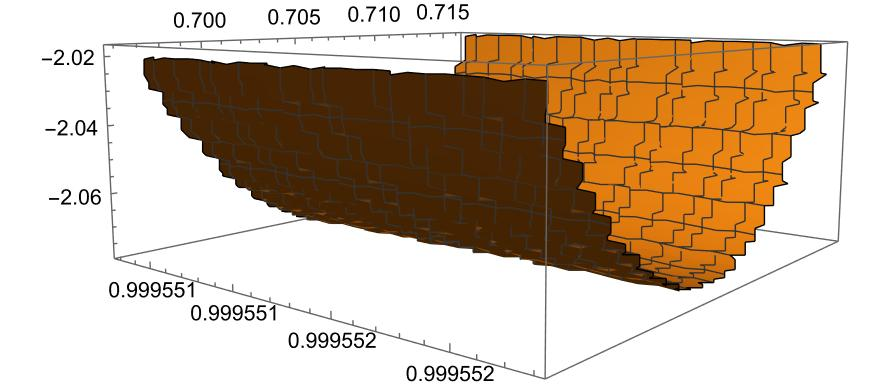
\includegraphics[width=0.8\linewidth]{fig/20240318.jpg}
  \caption{パラメターを??ととったときの最小値の候補}
  \label{fig:20240318}
\end{figure}















% ----------------------------------------
\clearpage
\bibliography{ref}
\bibliographystyle{ytamsalpha}

\nocite{Abe:2006xp}
\nocite{Abe:2007yb}
\nocite{Abe:2012ya}

\end{document}
